\section{Thực nghiệm và đánh giá}

\subsection{Giao diện hệ thống}

Hệ thống AVI được triển khai với hai giao diện chính: giao diện ứng dụng AVI trên máy tính (Hình \ref{c4:application}) được viết bằng PyQt5 và giao diện HMI trên dây chuyền (Hình \ref{c4:hmi}). Giao diện AOI cho phép hiển thị kết quả quá trình xử lý ảnh, là ảnh sau khi đã xử lý xong các bước align, crop và YOLO detect, các hộp bao từ mô hình YOLO cũng như kết quả đánh giá OK/NG của từng linh kiện. Người vận hành có thể phóng to, thu nhỏ, xem log xử lý theo thời gian thực và lưu toàn bộ ảnh phục vụ mục đích truy vết. Bên cạnh đó, giao diện HMI được thiết kế đơn giản hơn, phục vụ công nhân sản xuất, hiển thị trạng thái các thành phần trong hệ thống như trạng thái băng tải, trạng thái robot, tín hiệu cảm biến, số lượng sản phẩm OK/NG và các nút điều khiển như Start, Stop và Reset. Hai giao diện kết hợp giúp việc vận hành và giám sát hệ thống trở nên trực quan và thuận tiện.

\begin{figure}[H]
    \centering
    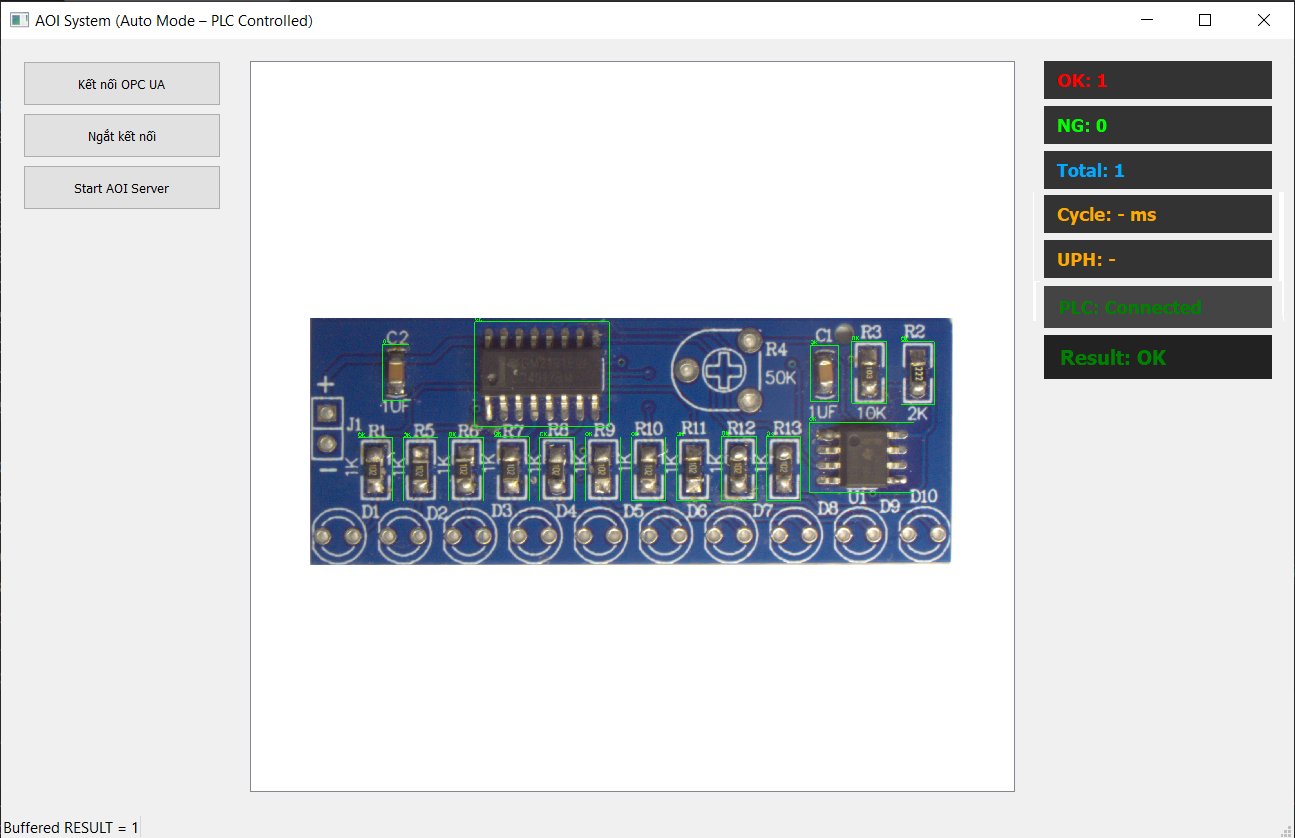
\includegraphics[width=1\linewidth]{figures/Chapter4/image1.png}
    \caption{Giao diện phần mềm AVI}
    \label{c4:application}
\end{figure}

\begin{figure}[H]
    \centering
    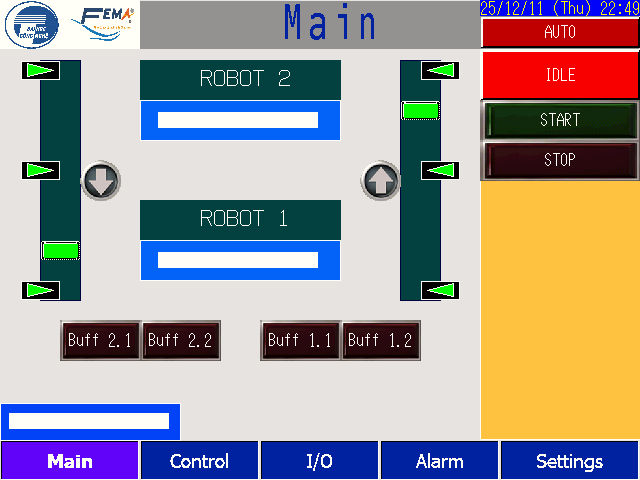
\includegraphics[width=0.8\linewidth]{figures/Chapter4/img2.jpg}
    \caption{Giao diện HMI}
    \label{c4:hmi}
\end{figure}


\begin{figure}[H]
    \centering
    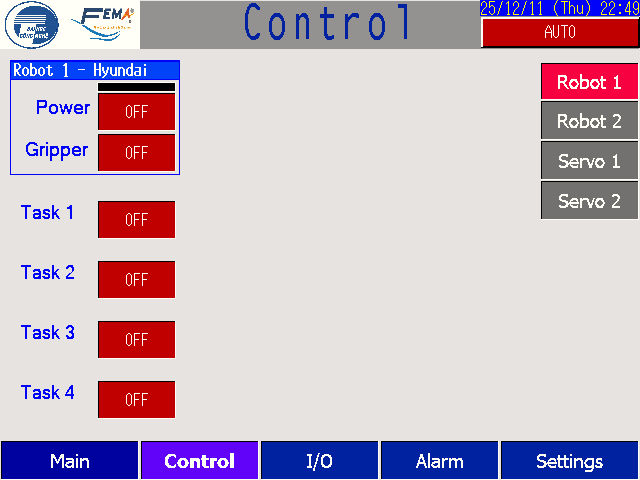
\includegraphics[width=0.48\linewidth]{figures/Chapter4/img1.jpg}
    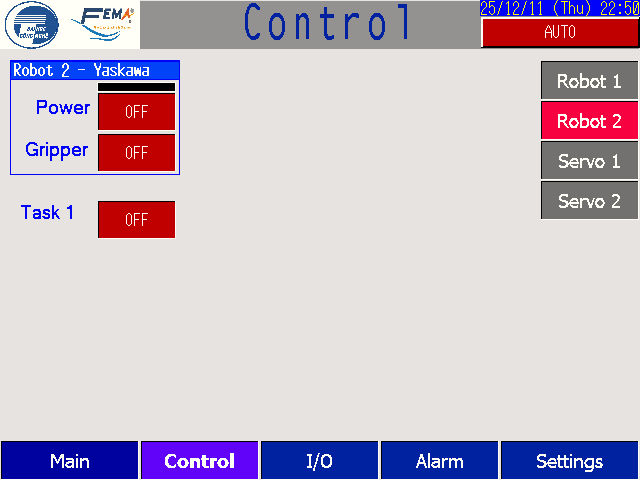
\includegraphics[width=0.48\linewidth]{figures/Chapter4/img3.jpg}
    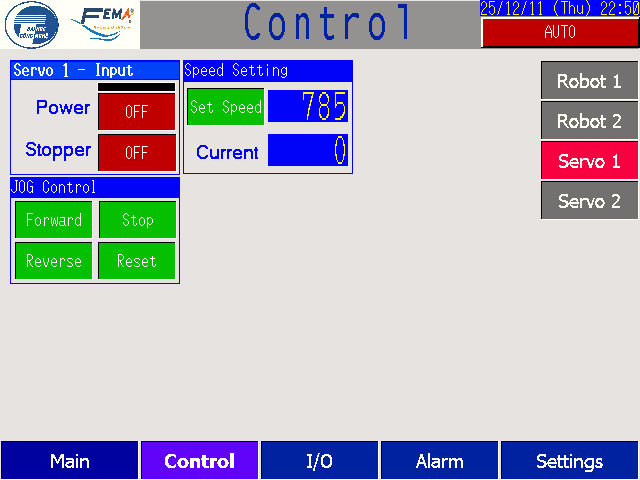
\includegraphics[width=0.48\linewidth]{figures/Chapter4/img4.jpg}
    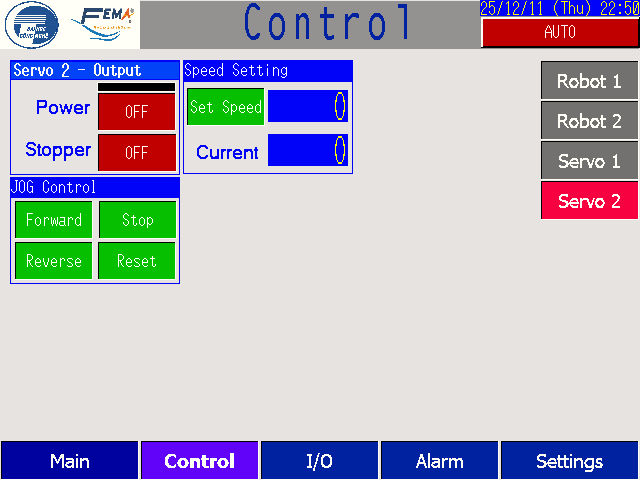
\includegraphics[width=0.48\linewidth]{figures/Chapter4/img5.jpg}
    \caption{Giao diện điều khiển Manual từng thành phần}
\end{figure}

\begin{figure}[H]
    \centering
    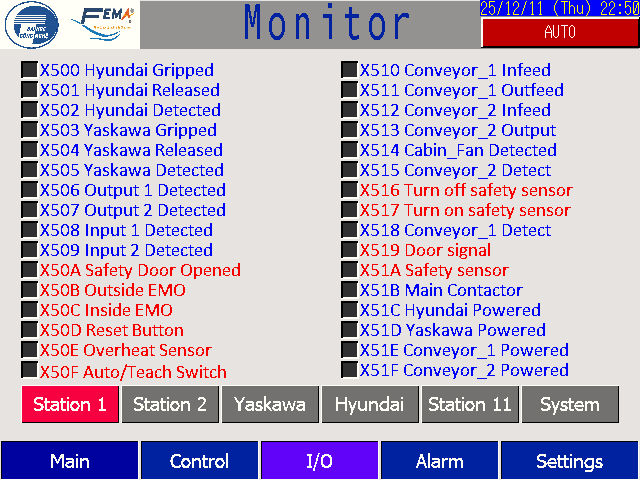
\includegraphics[width=0.48\linewidth]{figures/Chapter4/img6.jpg}
    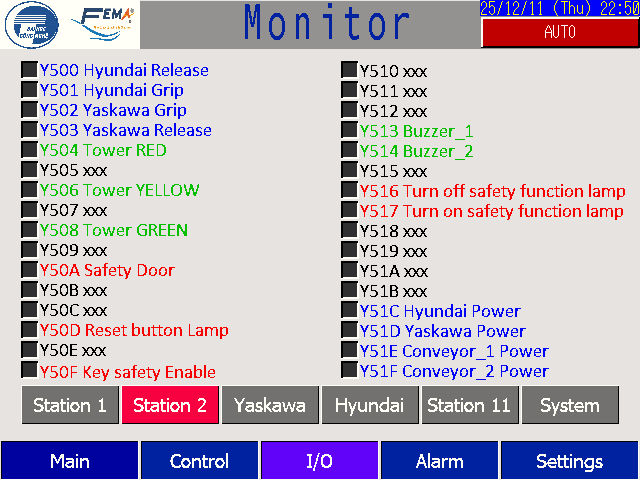
\includegraphics[width=0.48\linewidth]{figures/Chapter4/img7.jpg}
    \caption{Input/Output của hệ thống}
\end{figure}



\subsection{Kết quả nhận diện và phân loại sản phẩm}

Hình ảnh hệ thống sau khi lắp đặt:
\begin{figure}[H]
    \centering
    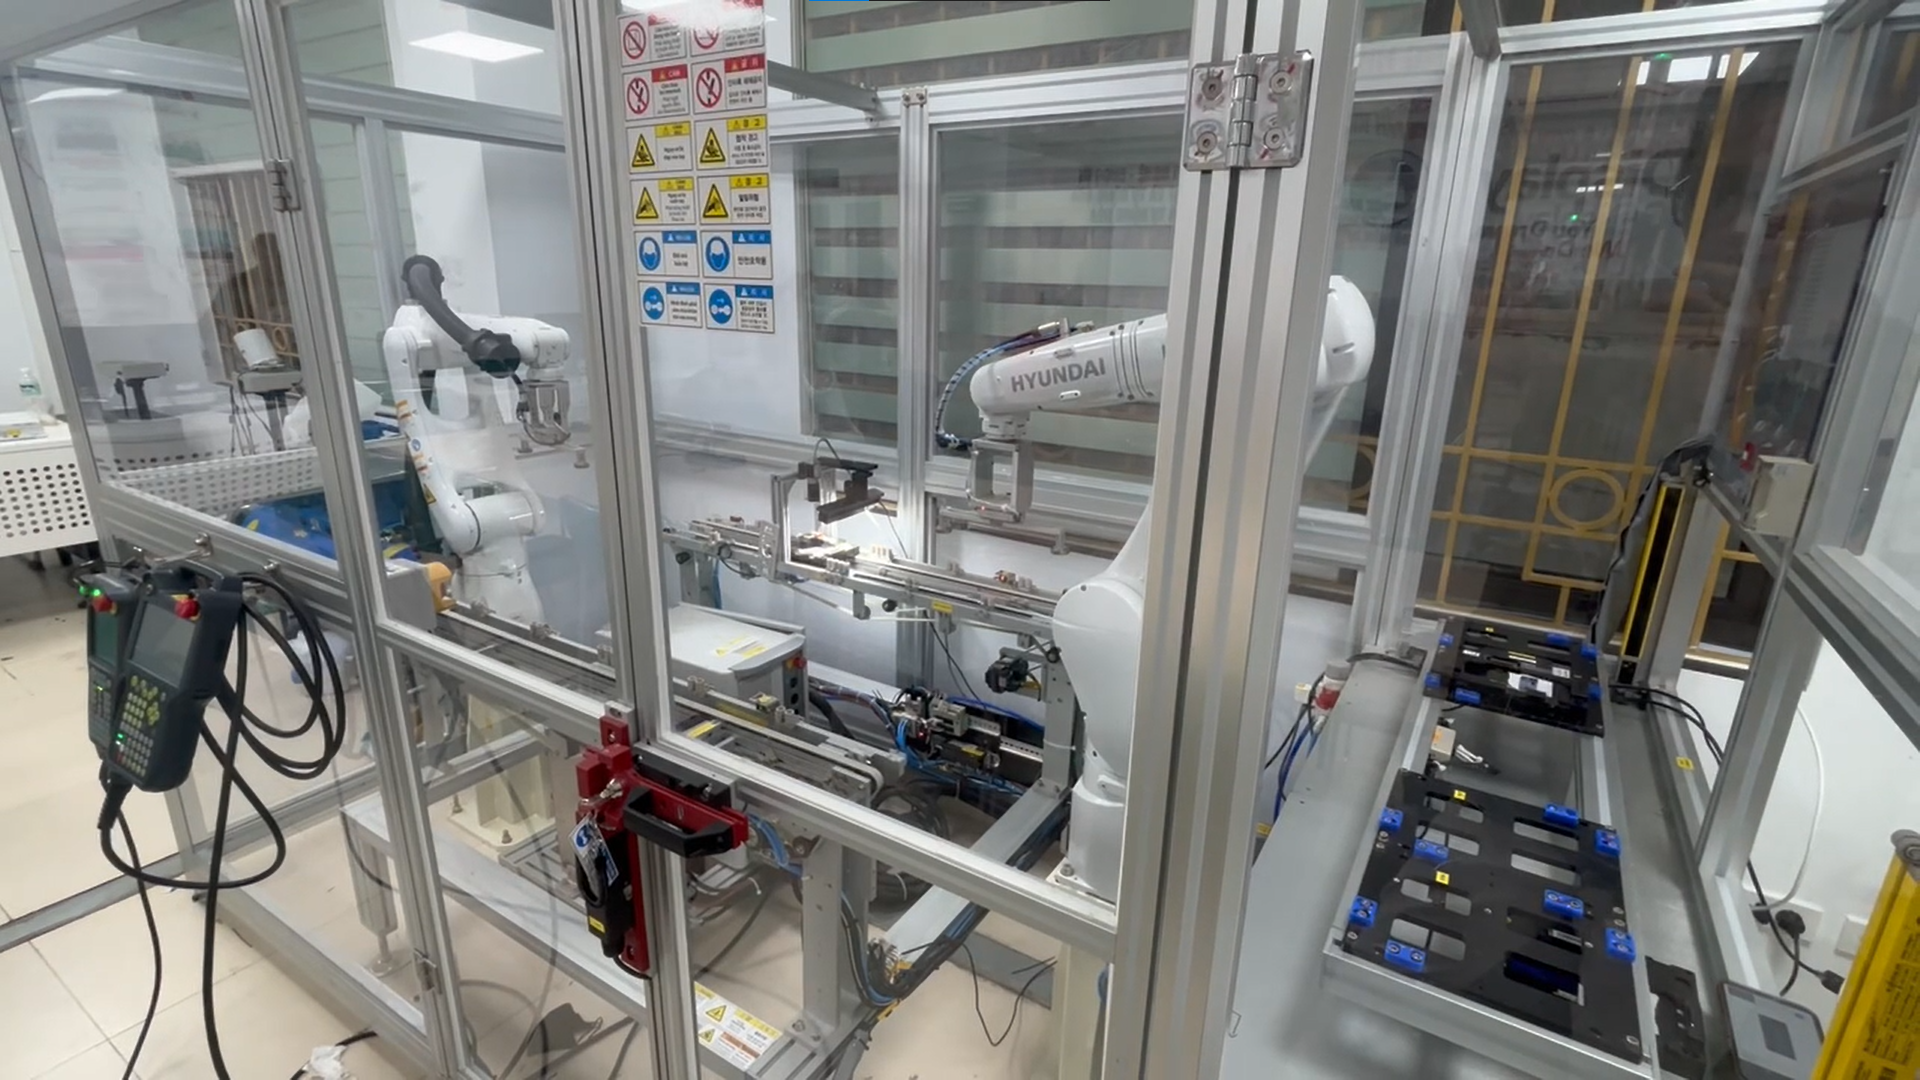
\includegraphics[width=1\linewidth]{figures/Chapter4/kq.png}
    \caption{Hệ thống thực tế}
\end{figure}

Hình ảnh giao diện ứng dụng khi hệ thống hoạt động:
\begin{figure}[H]
    \centering
    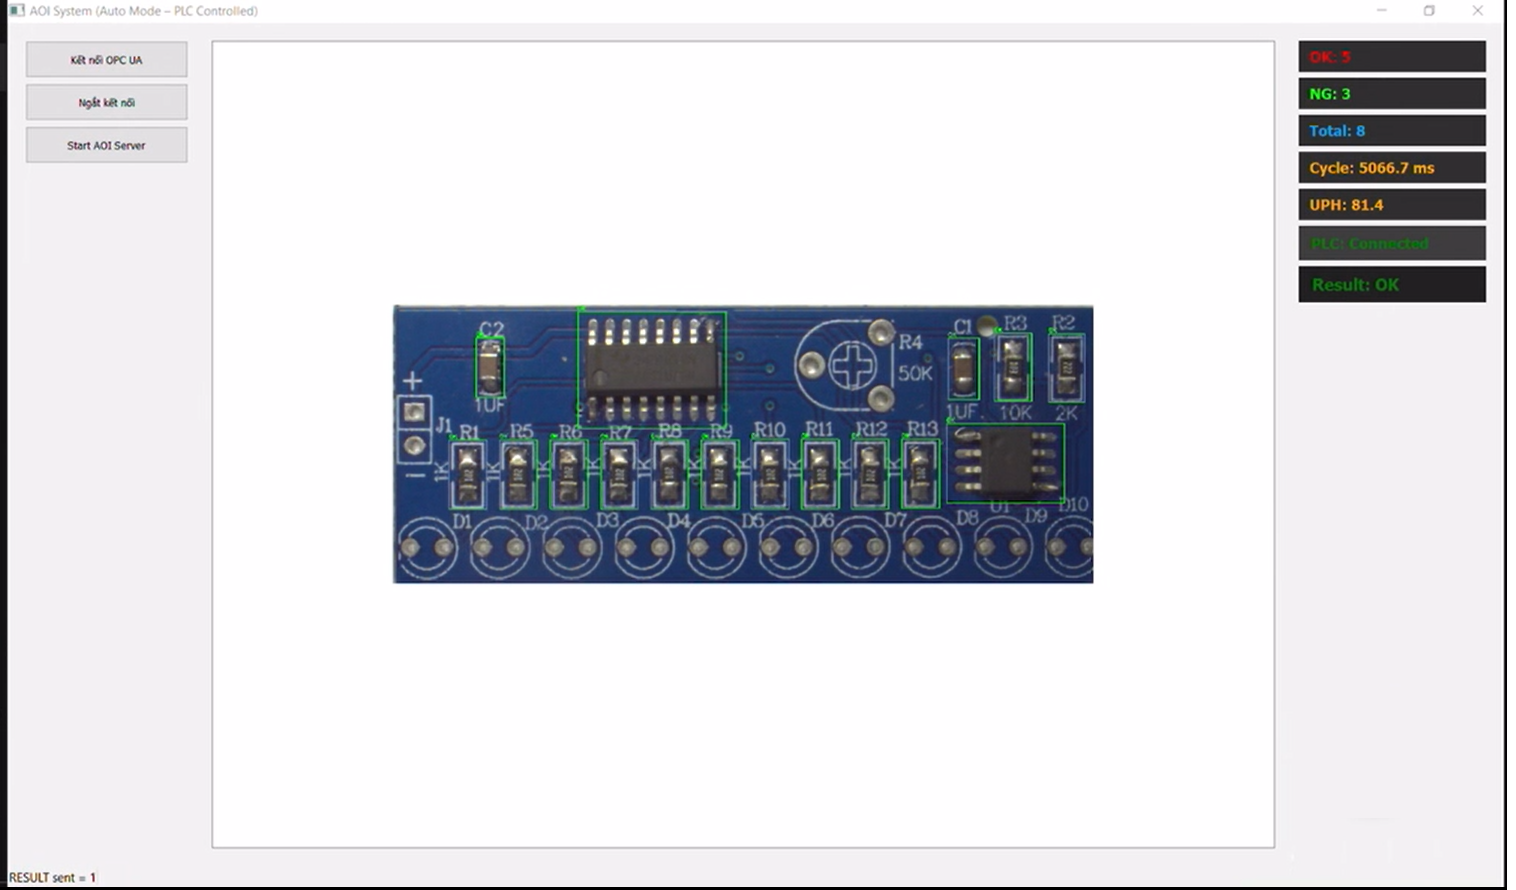
\includegraphics[width=1\linewidth]{figures/Chapter4/kq2.png}
    \caption{Kết quả hiển thị trên ứng dụng}
\end{figure}


Các thí nghiệm được thực hiện trên nhiều mẫu PCB bao gồm sản phẩm tốt và sản phẩm lỗi. Mô hình YOLO cho thấy khả năng nhận diện linh kiện SMD với độ chính xác cao, xác định đúng vị trí và loại linh kiện. Hệ thống phát hiện tốt các dạng lỗi phổ biến như thiếu linh kiện, lệch vị trí, xoay sai hướng và linh kiện sai loại. Các ảnh kết quả minh họa rõ vùng lỗi và hỗ trợ quá trình đánh giá sản phẩm.
Minh họa kết quả xử lý ảnh:
\begin{figure}[H]
    \centering
    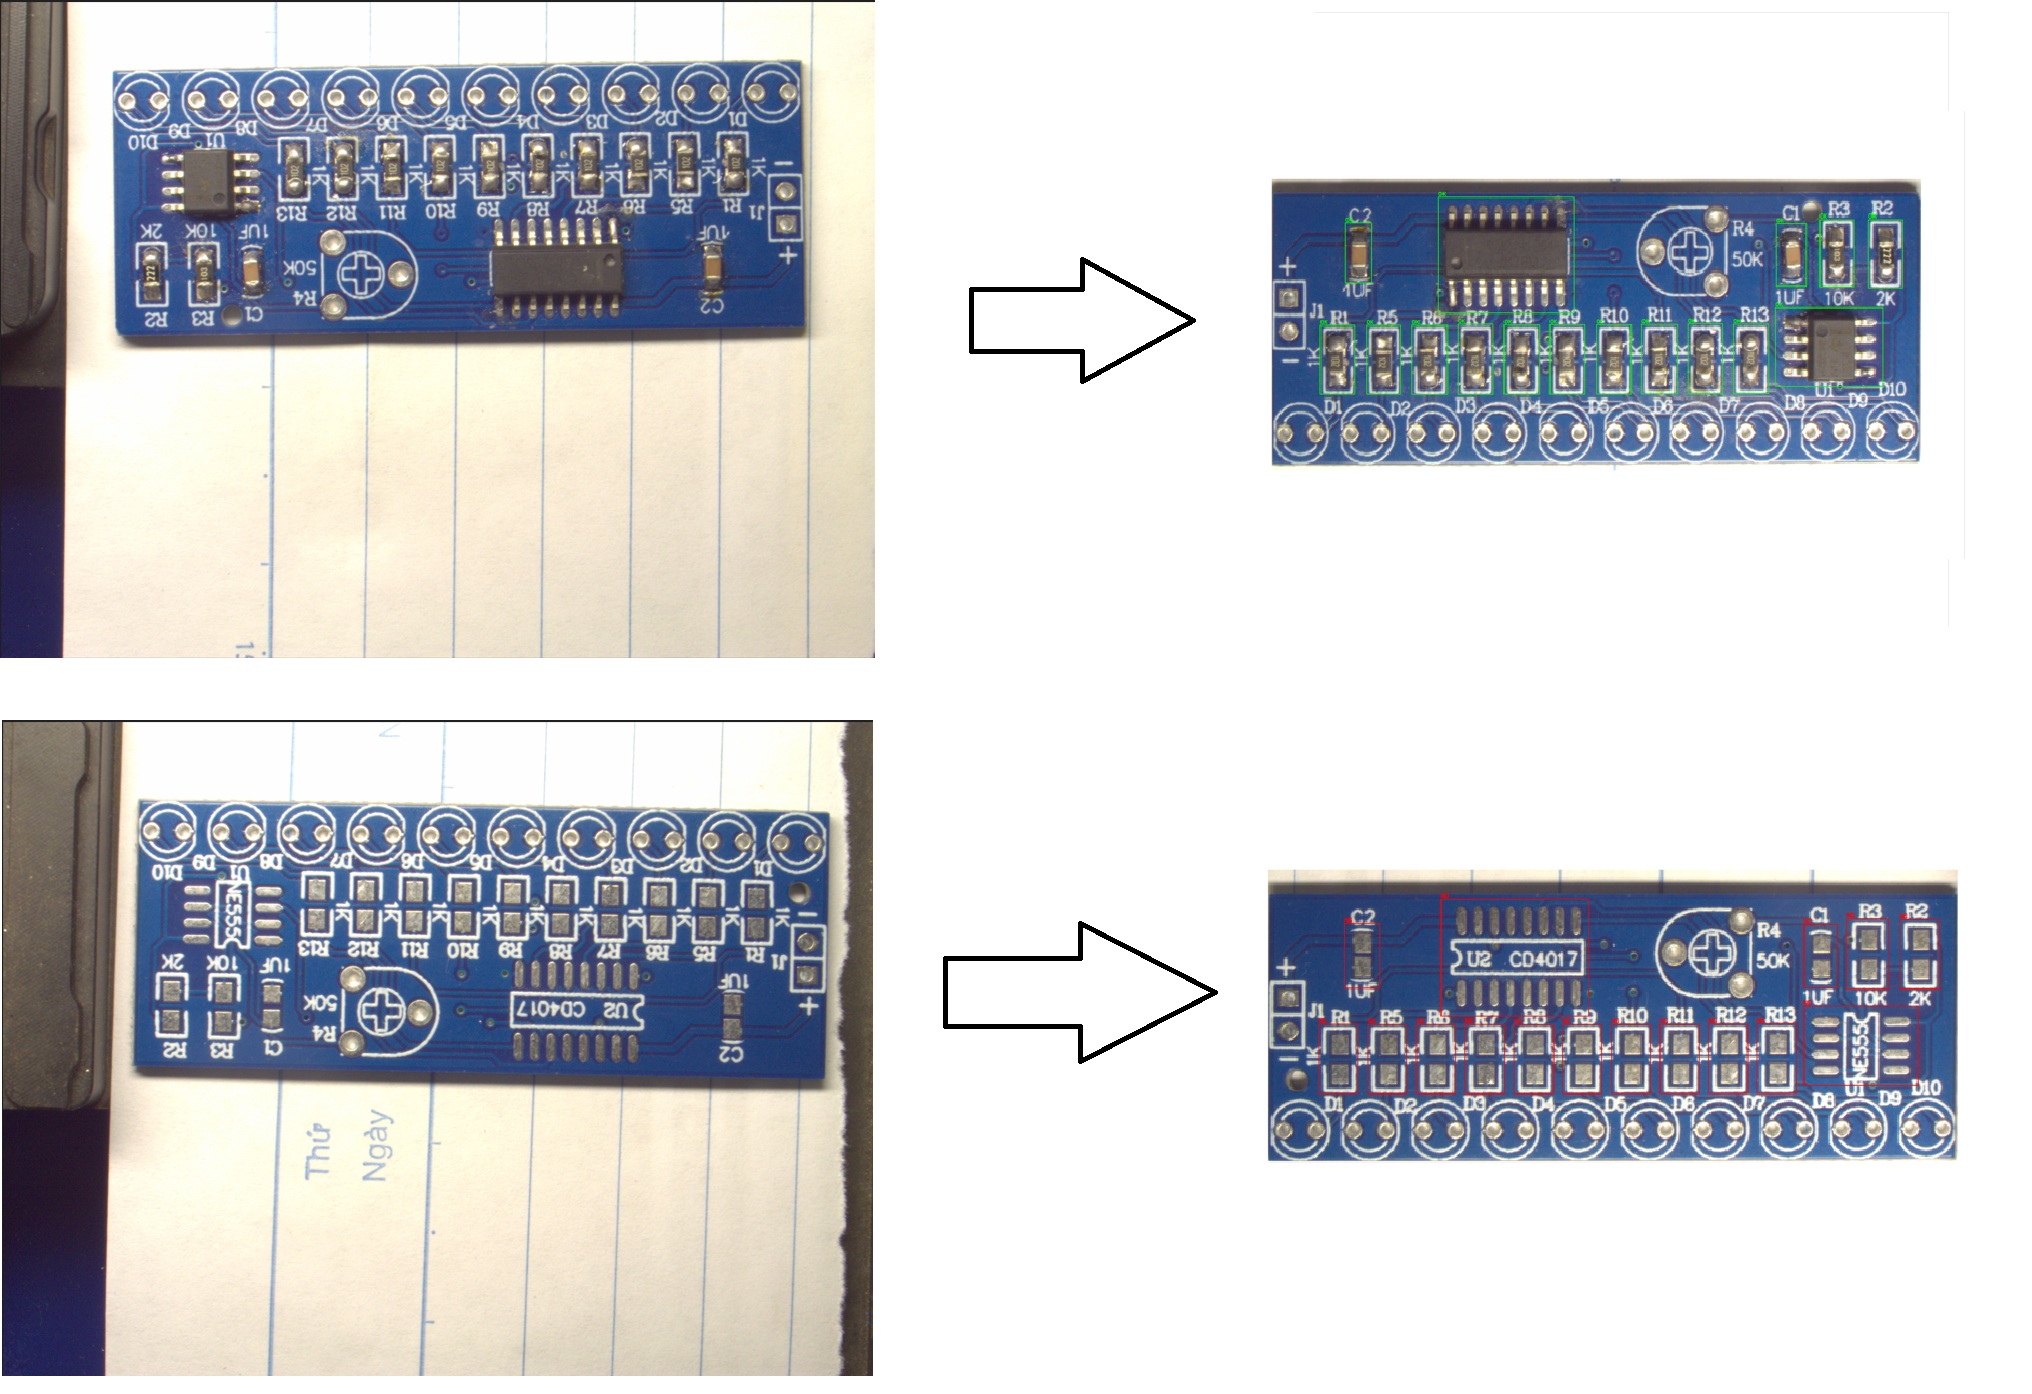
\includegraphics[width=1\linewidth]{figures/Chapter4/image3.png}
    \caption{Kết quả xử lý ảnh}
    \label{c4:image3}
\end{figure}


\subsection{Đánh giá hiệu suất: tốc độ, độ chính xác, độ ổn định}

Tốc độ xử lý trung bình của hệ thống đạt khoảng 3000--4000\,ms cho mỗi PCB, phụ thuộc nhiều vào phần cứng máy tính, đáp ứng tốt yêu cầu của dây chuyền sản xuất tốc độ cao. Độ chính xác nhận diện của mô hình YOLO đạt từ 95\% đến 98\%, trong khi các lỗi thiếu linh kiện được phát hiện với tỷ lệ 100\% Trong quá trình chạy liên tục nhiều giờ, hệ thống cho thấy tính ổn định cao, không phát sinh lỗi kết nối camera hoặc OPC UA.

\subsection{So sánh với phương pháp thủ công}

So với phương pháp kiểm tra thủ công bằng mắt thường, hệ thống AVI thể hiện ưu thế rõ rệt về tốc độ, độ chính xác và tính ổn định, đặc biệt khi sản phẩm cần kiểm tra có rất nhiều linh kiện nhỏ. Việc kiểm tra tự động giúp loại bỏ các sai sót chủ quan của người vận hành và phát hiện được những lỗi rất nhỏ mà mắt thường khó quan sát. Ngoài ra, hệ thống còn lưu trữ toàn bộ dữ liệu kiểm tra, hỗ trợ truy vết trong quá trình sản xuất. Do đó, phương pháp thủ công chỉ phù hợp cho kiểm tra mẫu hoặc sản lượng thấp, trong khi AVI là giải pháp tối ưu cho sản xuất hàng loạt.

\subsection{Cải tiến và nâng cấp}

Sau quá trình thiết kế và triển khai hệ thống kiểm tra ảnh tự động (AVI), có thể đề xuất một số hướng cải tiến nhằm nâng cao khả năng phát hiện lỗi, độ tin cậy và tính linh hoạt của hệ thống trong môi trường sản xuất thực tế.

\textbf{Thứ nhất}, cần mở rộng khả năng phát hiện nhiều loại lỗi hơn. Hệ thống hiện tại chủ yếu phát hiện các lỗi như thiếu linh kiện, lệch vị trí, xoay sai hướng và sai loại linh kiện. Để tăng cường hiệu quả kiểm tra, có thể bổ sung các lỗi nâng cao như dư linh kiện (gắn thừa), lệch quá giới hạn cho phép, sai giá trị linh kiện (ví dụ nhầm điện trở 1k và 10k), hoặc ngược cực linh kiện phân cực. Các lỗi này có thể được phát hiện bằng cách kết hợp kết quả từ mô hình YOLO với các thuật toán đo sai số hình học, phân loại patch bằng mạng CNN nhỏ, hoặc kiểm tra logic số lượng so với dữ liệu mẫu.

\textbf{Thứ hai}, hệ thống có thể được nâng cấp để hỗ trợ kiểm tra đa góc nhìn (6 sides inspection). Thay vì chỉ sử dụng ảnh chụp từ mặt trên (top view), có thể tích hợp thêm các camera ở cạnh bên hoặc góc nghiêng nhằm kiểm tra các mặt hông của linh kiện và bảng mạch. Phương pháp này giúp phát hiện các lỗi như thiếu chân IC, hàn dính cạnh, tụ bị ngẩng mặt (headstand), hoặc lỗi cơ khí mà ảnh mặt trên không thể quan sát được. Việc xử lý ảnh từ nhiều góc nhìn có thể được thực hiện bằng cách huấn luyện các mô hình riêng biệt cho từng camera hoặc sử dụng kỹ thuật căn chỉnh ảnh (warp perspective) trước khi xử lý.

\textbf{Thứ ba}, cần tích hợp thêm phương pháp phát hiện bất thường (anomaly detection) để xử lý các lỗi không lường trước hoặc không có sẵn nhãn huấn luyện. Trong môi trường sản xuất đa dạng, không thể liệt kê hết mọi dạng lỗi, đặc biệt là các lỗi hiếm. Do đó, sử dụng các mô hình học không giám sát như Autoencoder, PatchCore, hoặc PaDiM có thể giúp phát hiện các điểm bất thường dựa trên sai lệch phân phối đặc trưng so với mẫu chuẩn. Các kỹ thuật này có thể tạo ra bản đồ nhiệt (heatmap) vùng lỗi, giúp người vận hành nhận diện và đánh giá nguyên nhân nhanh chóng.

\textbf{Thứ tư}, giao diện người dùng (GUI) có thể được mở rộng để hỗ trợ các chức năng nâng cao như hiển thị phân tích lỗi theo thời gian thực, cho phép người dùng chọn chế độ kiểm tra (YOLO hoặc anomaly), truy xuất lại ảnh lỗi, và tự động lưu log kiểm tra theo batch sản xuất. Điều này không chỉ nâng cao trải nghiệm vận hành mà còn hỗ trợ quá trình truy vết và cải tiến chất lượng.

Tổng thể, các cải tiến trên góp phần nâng cao khả năng phát hiện lỗi toàn diện, tăng độ tin cậy của hệ thống trong các tình huống phức tạp, đồng thời tạo nền tảng để phát triển một hệ thống AVI linh hoạt, thông minh và có khả năng mở rộng trong tương lai.
